\section{Results \& Discussion}
For all of the following simulations, we set the value of the parameters to $a=3$, $b=0.1$ and $c=1$ with the initial condition of $(X_0,Y_0,Z_0)=(2,3,2)$. As the numerical method used to solve the fractional-order equations needs a certain time of simulation ($T$) and number of iterations ($N$) it was used $N=10000$ and $T=1000$ thus the time-step is $0.1$. It is important to highlight, that the results of the simulation are strongly dependent of the value of the last conditions to obtain the same result as the presented in this article.  
\subsection{Comparison between Chen's paper and results obtained}
\subsubsection{Equal fractional order system}
\begin{figure}[H]
  \centering
  \begin{subfigure}[H]{0.4\textwidth}
    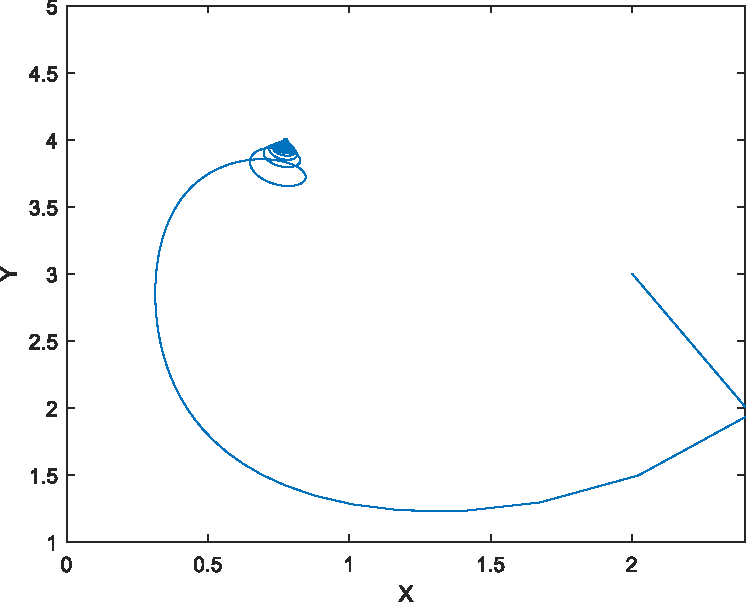
\includegraphics[scale = 0.5]{files/a084.pdf}
    \centering
    \caption{Results when $\alpha=0.84$.}
    \label{fig:2a}
  \end{subfigure}
  \hspace{1cm}
  \begin{subfigure}[H]{0.4\textwidth}
    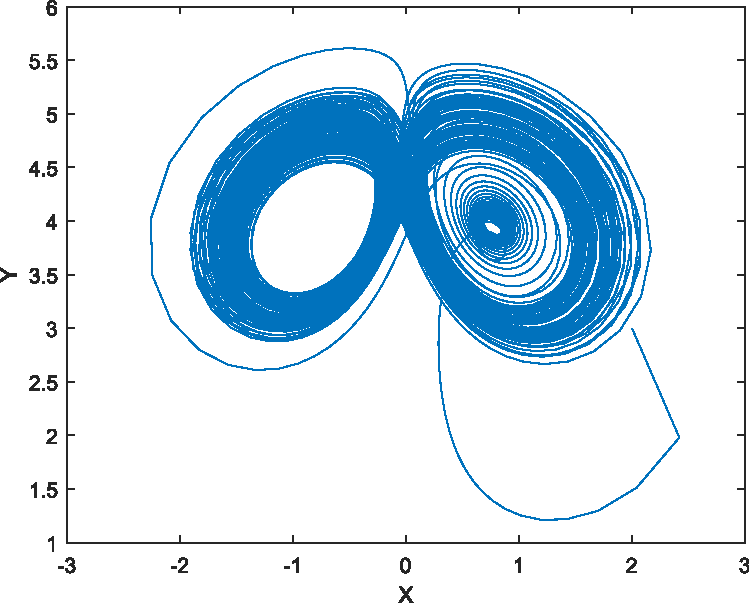
\includegraphics[scale = 0.5]{files/b085.pdf}
    \centering
    \caption{Results when $\alpha=0.85$.}
    \label{fig:2b}
  \end{subfigure}
  \caption{Results for equal fractional order system when $q_1=q_2=q_3=\alpha$.}
  \label{img:equalalpha}
\end{figure}


In figure \ref{img:equalalpha}, the results for equal fractional order are shown. These plots are comparable with the ones showed in Chen's paper \cite{main} in figure \ref{img:equalalpha} (a-b). On the figure \ref{fig:2a}, it can be observed that the plots are slightly different. On the other hand, on figure \ref{fig:2b} the shape is highly similar to the original but, the filling of the graph is not comparable. It would be explained later why this dissimilarities occur. Note that the system changes from a stable trajectory to a chaotic one with a small change on the order. This result will be discussed in the stability analysis section.

\subsubsection{Non-equal fractional order systems}
\begin{figure}[H]
        \centering
        \begin{subfigure}[b]{0.475\textwidth}
            \centering
            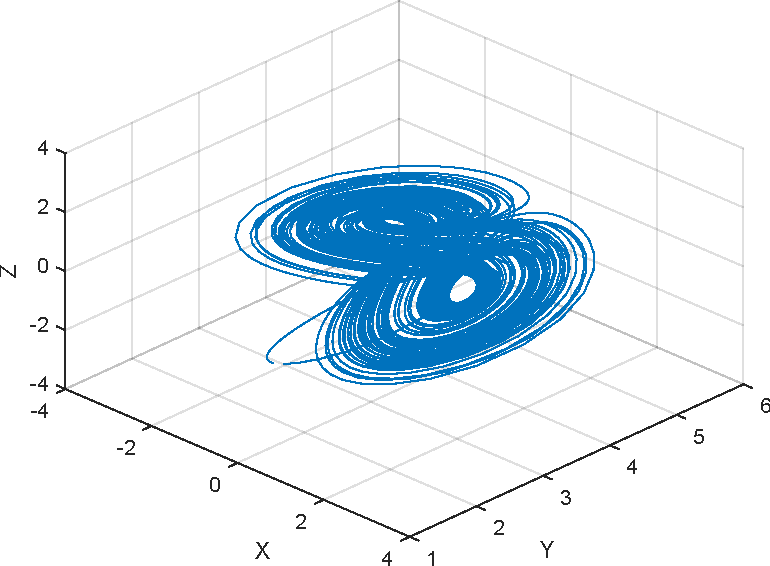
\includegraphics[scale=0.5]{files/a_0_9_1_1.pdf}
            \caption{$q_1=0.90$}    
            \label{fig:3a}
        \end{subfigure}
        \hfill
        \begin{subfigure}[b]{0.475\textwidth}  
            \centering 
            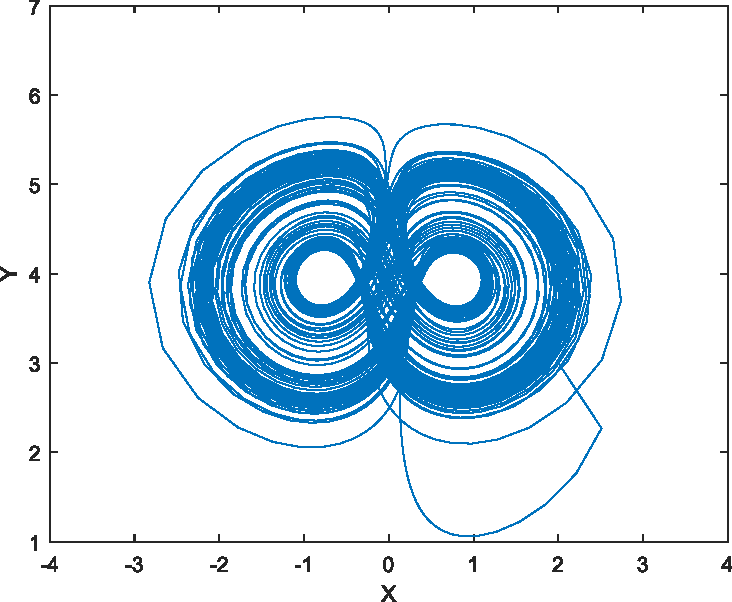
\includegraphics[scale=0.5]{files/b080_1_1.pdf}
            \caption{$q_1=0.80$}  
            \label{fig:mean and std of net24}
        \end{subfigure}
        \vskip\baselineskip
        \begin{subfigure}[b]{0.475\textwidth}   
            \centering 
            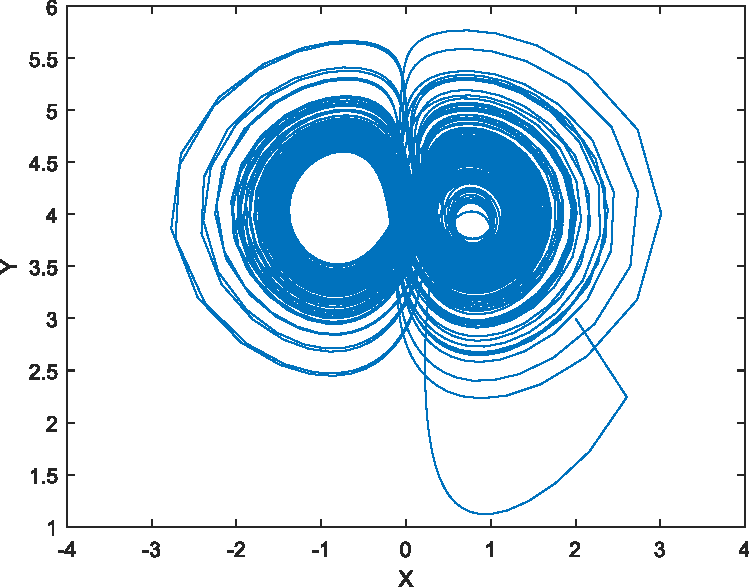
\includegraphics[scale=0.5]{files/c_070_1_1.pdf}
            \caption{$q_1=0.70$}    
            \label{fig:mean and std of net34}
        \end{subfigure}
        \quad
        \begin{subfigure}[b]{0.475\textwidth}   
            \centering 
            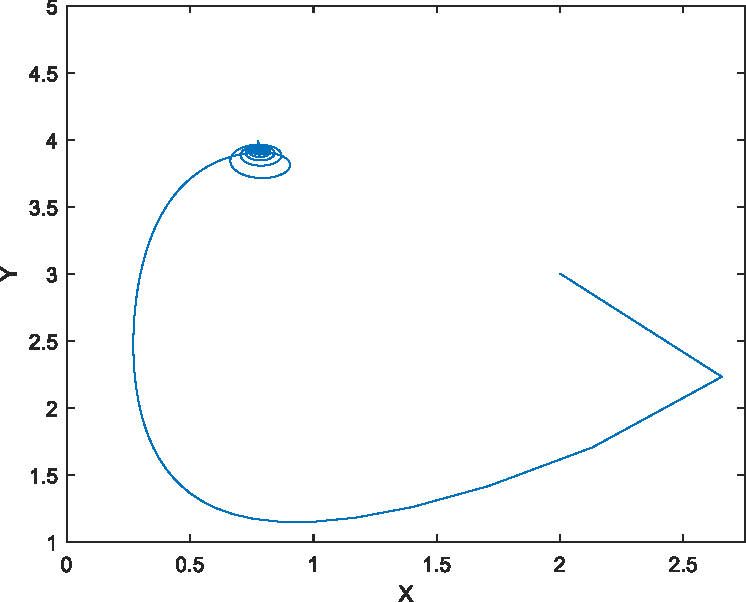
\includegraphics[scale=0.5]{files/d_065_1_1.pdf}
            \caption{$q_1=0.65$}   
            \label{fig:3d}
        \end{subfigure}
        \caption{Results for $q_2=q_3=1$} 
        \label{fig:q2eqq3}
	\end{figure}
In figure, \ref{fig:3a} it was shown the third-dimensional graph instead of a phase-state plane just for illustration purposes. On the remaining it can be seen their similitude with Chen's article.

\begin{figure}[H]
  \centering
  \begin{subfigure}[H]{0.4\textwidth}
    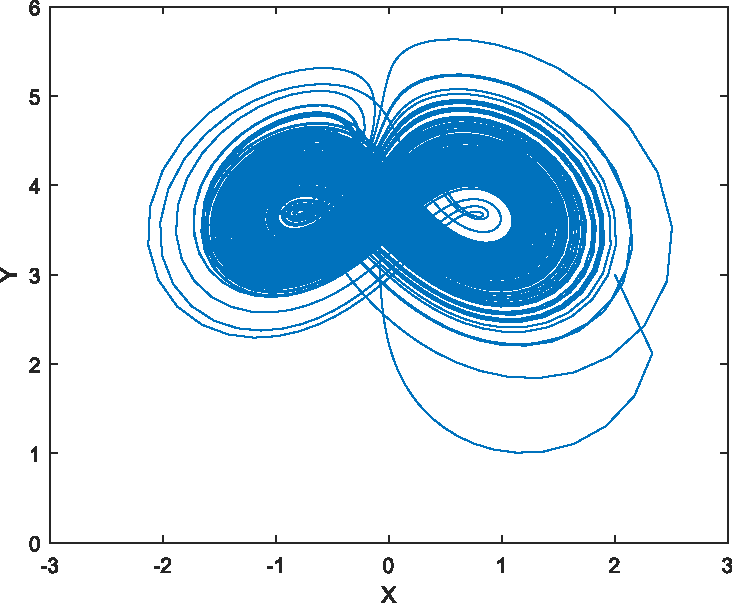
\includegraphics[scale = 0.5]{files/c_1_090_1.pdf}
    \centering
    \caption{$q_2=0.90$.}
  \end{subfigure}
  \hspace{1cm}
  \begin{subfigure}[H]{0.4\textwidth}
    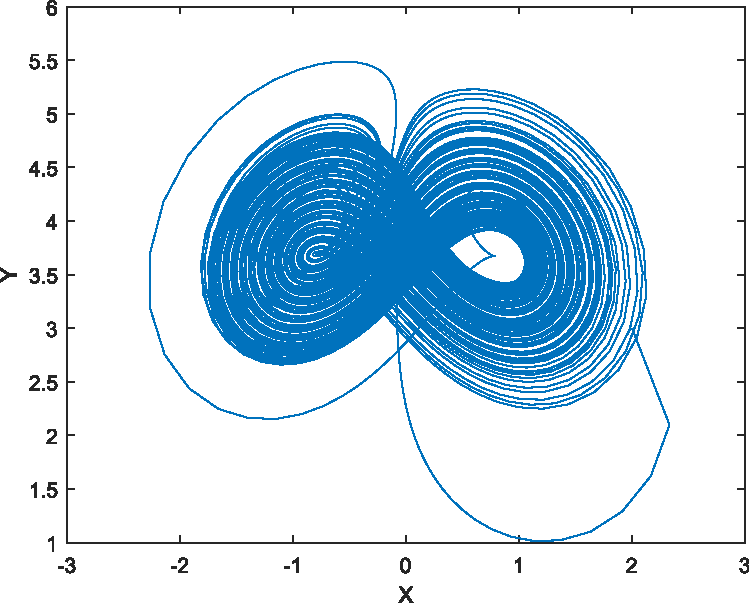
\includegraphics[scale = 0.5]{files/d_1_089_1.pdf}
    \centering
    \caption{$q_2=0.89$.}
    \label{img:messed}
  \end{subfigure}
  \caption{Results for $q_1=q_3=1$.}
  \label{img:q1eqq3}
\end{figure}
Figures \ref{img:q1eqq3}(a-b) are matched to the Figures 3(c-d) in Chen's paper. It can be seen that both graphics are quite different to the ones presented at the original article. Figure \ref{img:messed} graphic has the most considerable difference; even though, it preserves the uniformity of the graph.

\begin{figure}[H]
        \centering
        \begin{subfigure}[b]{0.475\textwidth}
            \centering
            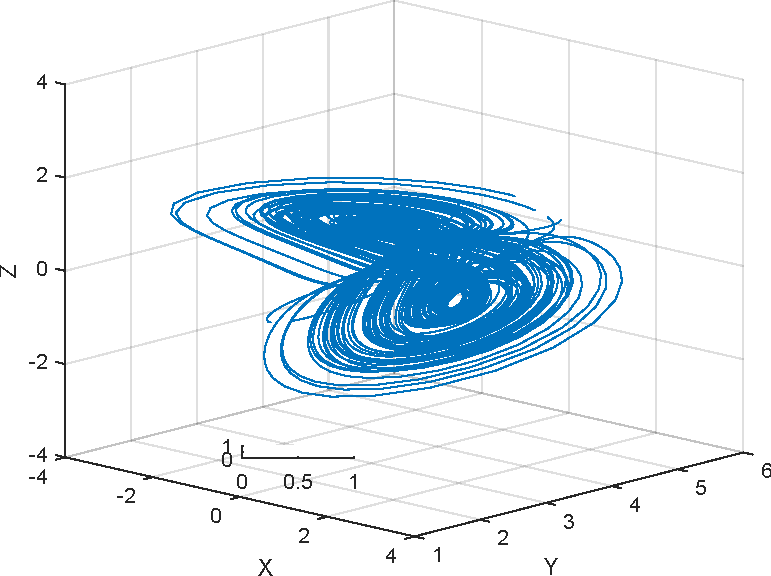
\includegraphics[scale=0.5]{files/a_1_1_090.pdf}
            \caption{$q_3=0.90$}    
            \label{fig:mean and std of net14}
        \end{subfigure}
        \hfill
        \begin{subfigure}[b]{0.475\textwidth}  
            \centering 
            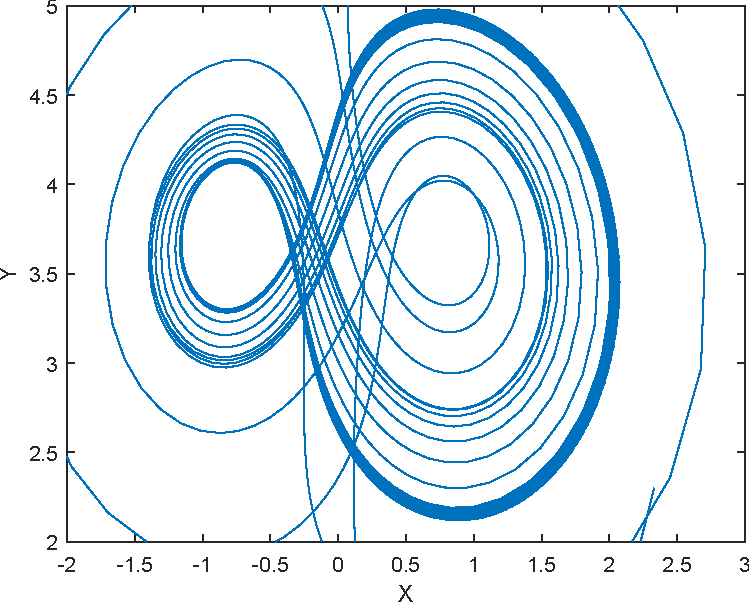
\includegraphics[scale=0.5]{files/b_1_1_080.pdf}
            \caption{$q_3=0.80$}  
            \label{fig:messed2}
        \end{subfigure}
        \vskip\baselineskip
        \begin{subfigure}[b]{0.475\textwidth}   
            \centering 
            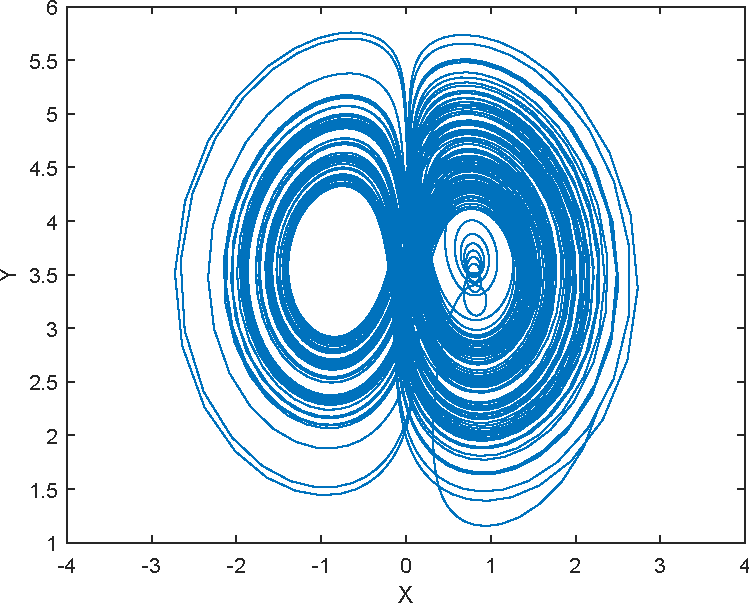
\includegraphics[scale=0.5]{files/c_1_1_05.pdf}
            \caption{$q_3=0.70$}    
            \label{fig:mean and std of net34}
        \end{subfigure}
        \quad
        \begin{subfigure}[b]{0.475\textwidth}   
            \centering 
            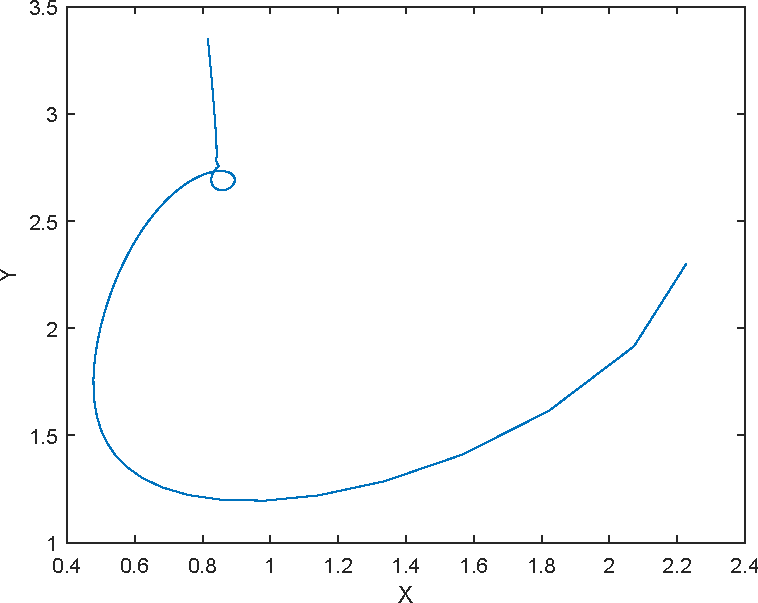
\includegraphics[scale=0.5]{files/d_1_1_020.pdf}
            \caption{$q_3=0.20$}   
            \label{fig:5d}
        \end{subfigure}
        \caption{Results for $q_1=q_2=1$} 
        \label{fig:q1eqq2}
	\end{figure}
    All of the figures depicted at Figure \ref{fig:q1eqq2} are associated to the 5th Figure of Chen. It can be perceived that all of the plots shown above are interchangeable one another with the exception of Figure \ref{fig:messed2}. But, the chart mentioned preserves the shape of the primal.
    
    The differences of the above phase-state portraits could be explained by a number of causes. First of all, Chen does not specifies the time-step nor the upper-bound of the time interval about the simulation that they run; therefore, the lines in the plots can have more iterations thus have more trajectories. On the other hand, Figures \ref{fig:2a}, \ref{fig:3d} or \ref{fig:5d} as they converge to one specific point, it is not as dependent of the time iterations as the rest, therefore their similitude with the original is almost perfect. Another cause for this difference is that the modifications for the Adams-Bashforth-Moulton predictor-corrector, recommended in \cite{diethelm2002predictor}, were not applied for the simulations. It is important to highlight that small changes on the system's order lead to big changes on its behavior.

\subsection{Comparison between Runge-Kutta method and Adams-Bashforth-Moulton predictor-corrector}

In this section, it will be compared the results that both methods give using integer order differentiation. The parameters $a=b=c=0$ were used, therefore the figure \ref{fig:6} can be compared to the second figure of article \cite{integrability}. In the figure \ref{fig:6} the initial conditions were $(x_0,y_0,z_0)=(0,0,2.21)$ and for the next ones, $(x_0,y_0,z_0)=(0,0,1.6)$ was used.

\begin{figure}[H]
  \centering
  \begin{subfigure}[H]{0.4\textwidth}
    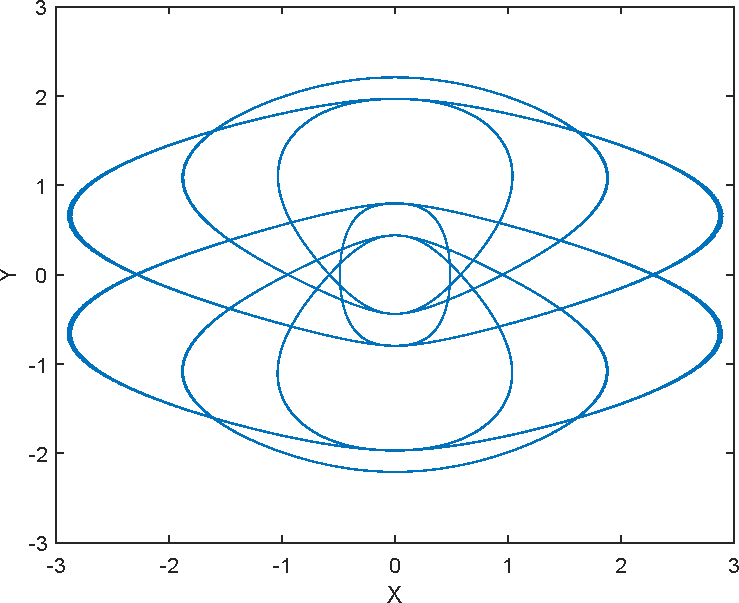
\includegraphics[scale = 0.5]{files/IntegerKutta.pdf}
    \centering
    \caption{Results using Runge-Kutta method.}
  \end{subfigure}
  \hspace{1cm}
  \begin{subfigure}[H]{0.4\textwidth}
    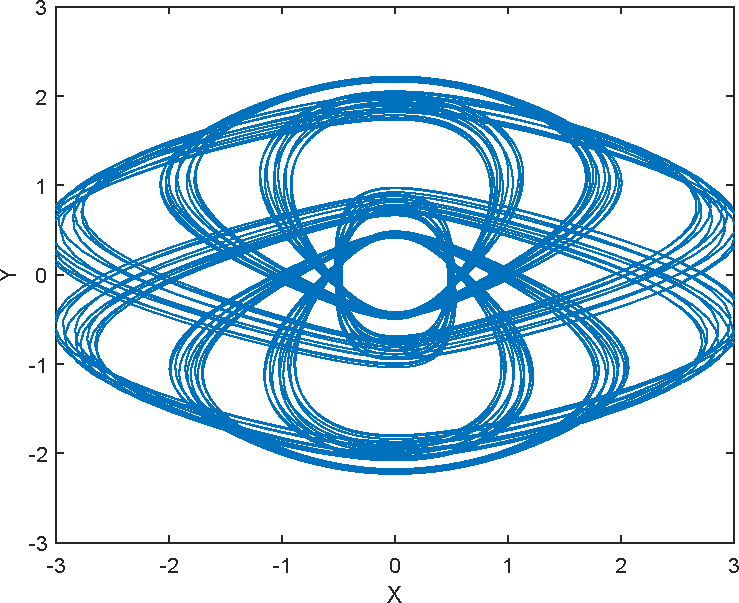
\includegraphics[scale = 0.5]{files/IntegerAdams.pdf}
    \centering
    \caption{Results using Adams-Bashforth-Moulton predictor-corrector.}
    \label{}
  \end{subfigure}
  \caption{Results for integer-order system, i.e. $q_1=q_2=q_3=1$}
  \label{fig:6}
\end{figure}

\begin{figure}[H]
  \centering
  \begin{subfigure}[H]{0.4\textwidth}
    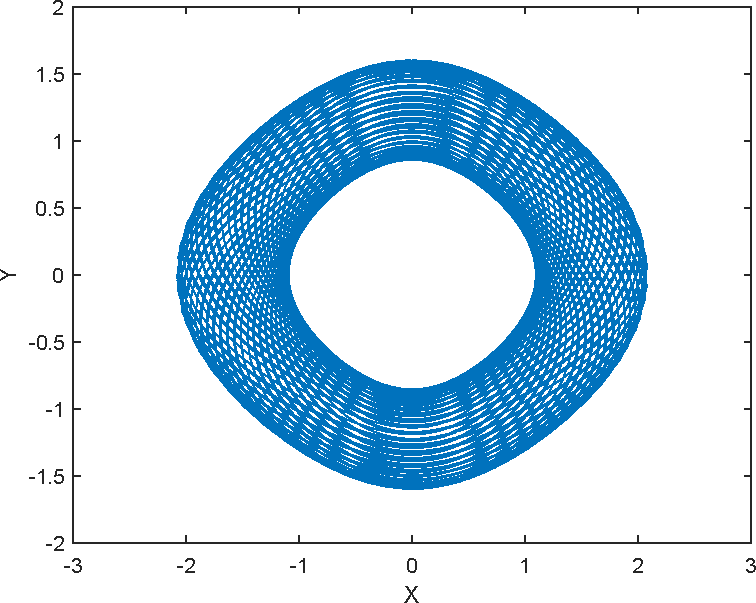
\includegraphics[scale = 0.5]{files/IntegerKutta2.pdf}
    \centering
    \caption{Results using Runge-Kutta method.}
  \end{subfigure}
  \hspace{1cm}
  \begin{subfigure}[H]{0.4\textwidth}
    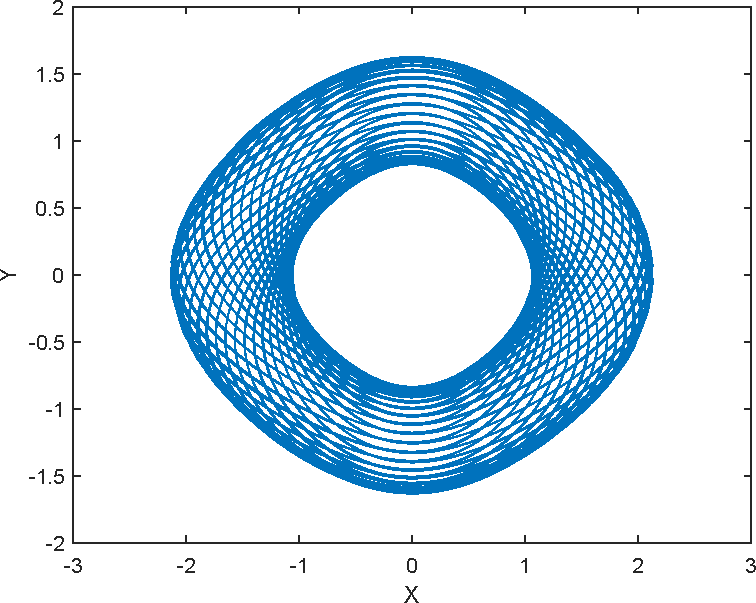
\includegraphics[scale = 0.5]{files/IntegerAdam2.pdf}
    \centering
    \caption{Results using Adams-Bashforth-Moulton predictor-corrector.}
    \label{}
  \end{subfigure}
  \caption{Results for integer-order system, i.e. $q_1=q_2=q_3=1$}
  \label{fig:7}
\end{figure}

It can be shown that both graphs keep the same form independently of the method used; as explained before, the Runge-Kutta is more precise than the other numerical method due to the difference of order. Therefore, every discrepancy of the plots can be explained with the above. 
